% Layout check for the paper's figures and tables in the IEEE conference template.
% Overleaf: upload this file, tables.tex, Fig1.pdf and Fig2.pdf to one project and compile
% with pdfLaTeX (IEEEtran.cls is built in). Copy the figure blocks below into the paper.
\documentclass[conference]{IEEEtran}
\usepackage{graphicx}
\usepackage{booktabs}
\usepackage{amssymb}

\begin{document}
\title{Float layout check}
\maketitle

\section{Figures}

% Fig. 1: two-column width (6.2 x 2.5 in), place near Section IV-A.
\begin{figure*}[t]
\centering
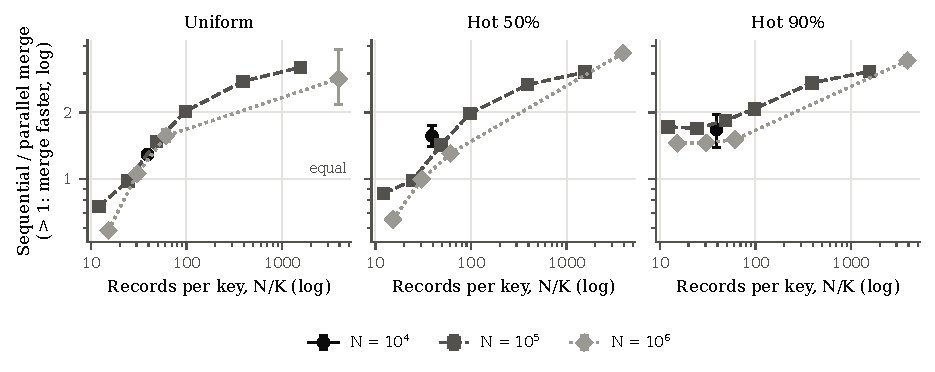
\includegraphics[width=0.9\textwidth]{Fig1.pdf}
\caption{Sequential time divided by parallel-merge time versus records per key ($N/K$) on platform A, for uniform, 50\%-hot and 90\%-hot inputs. Lines connect observed points; error bars span the ratio of the two methods' individual 99.9\% interval end points and are not a confidence interval of the ratio. The $N{=}10^4$, 90\%-hot point (1.68) is the original measurement; a re-measurement with a longer warm-up gave 1.35 (Section IV-E).}
\label{fig:crossover}
\end{figure*}

% Fig. 2: one-column width (3.4 x 3.2 in), place near Section IV-B.
\begin{figure}[t]
\centering
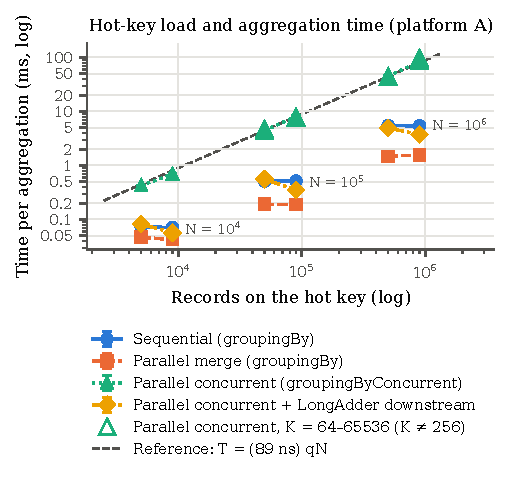
\includegraphics[width=\columnwidth]{Fig2.pdf}
\caption{Time per aggregation versus records on the hot key for $K{=}256$ on platform A (log--log). Hollow triangles: parallel concurrent grouping at other $K$. Dashed line: median normalized cost (89\,ns per hot-key record). The \texttt{LongAdder} series is the control, not a stock collector; its slow configurations at other $K$ are listed in Table~\ref{tab:exceptions}.}
\label{fig:skew}
\end{figure}

\section{Tables}
Tables \ref{tab:platforms}, \ref{tab:downstream}, \ref{tab:exceptions} and \ref{tab:guide}.

% Tables for "When Concurrent Is Slower: Hot Keys and Java Stream Grouping Collectors"
% Source of every number: 논문초안_KR.md (Tables I-IV) and 결과분석표.md.
% IEEEtran numbers tables in the order their \caption appears in the source, so place
% each table right after the paragraph that first cites it: I (III-C), II (IV-C),
% III (IV-D), IV (IV-F). Refer to them with \ref{tab:...}.
%
% Preamble:
%   \usepackage{booktabs}   % \toprule, \midrule, \bottomrule
%   \usepackage{amssymb}    % \gtrsim, \lesssim (Table IV)

% ---------------------------------------------------------------- Table I (one column)
\begin{table}[t]
\caption{Evaluation platforms}
\label{tab:platforms}
\centering
\footnotesize
\setlength{\tabcolsep}{3pt}
\begin{tabular}{@{}p{1.45cm}p{3.05cm}p{3.35cm}@{}}
\toprule
 & Platform A & Platform B \\
\midrule
CPU & Apple M5 (4 performance + 6 efficiency cores) & Intel Core i5-8250U (4 cores, 8 threads, 6\,MiB L3) \\
Memory & 32\,GiB & 20\,GB DDR4 \\
OS & macOS 26.6.2 & Ubuntu 24.04.2 (Linux 6.14) \\
JDK & Temurin 25.0.4.1 & Temurin 25.0.4.1 \\
Cores & not pinned & pinned to CPUs 0--3 (one per physical core) \\
\midrule
Common & \multicolumn{2}{p{6.5cm}@{}}{JMH 1.37; heap 512\,MiB; common-pool parallelism 3; warm-up 5$\times$1\,s, measurement 5$\times$1\,s, 3 JVM forks} \\
\bottomrule
\end{tabular}
\end{table}

% ---------------------------------------------------------------- Table II (one column)
\begin{table}[t]
\caption{Downstream implementations on platform A ($N{=}10^5$, $K{=}256$, one session). Time in ms $\pm$ JMH 99.9\% interval}
\label{tab:downstream}
\centering
\footnotesize
\setlength{\tabcolsep}{2.5pt}
\begin{tabular}{@{}llllr@{}}
\toprule
Downstream & Per-key & Counter & \multicolumn{2}{c@{}}{Hot-key share} \\
\cmidrule(l){4-5}
 & monitor & & 50\% & 90\% \\
\midrule
\texttt{counting()}$^{a}$ & yes & \texttt{long[]} & 4.46$\pm$0.09 & 7.84$\pm$0.33 \\
\texttt{syncAtomic} & yes & \texttt{AtomicLong} & 4.19$\pm$0.06 & 3.97$\pm$0.42 \\
\texttt{syncAdder} & yes & \texttt{LongAdder} & 4.74$\pm$0.26 & 4.30$\pm$0.55 \\
\texttt{casAtomic} & no & \texttt{AtomicLong} & 1.58$\pm$0.01 & 2.29$\pm$0.03 \\
\texttt{casAdder}$^{b}$ & no & \texttt{LongAdder} & 0.55$\pm$0.02 & 0.35$\pm$0.02 \\
\bottomrule
\end{tabular}
\par\smallskip
\parbox{\linewidth}{\scriptsize $^{a}$Stock collector. $^{b}$Control. \texttt{sync*}: downstream without \texttt{CONCURRENT}, so the JDK adds a per-key \texttt{synchronized} block; \texttt{cas*}: same accumulator with \texttt{CONCURRENT}. Under the monitor the \texttt{LongAdder} created no cells.}
\end{table}

% ---------------------------------------------------------------- Table III (two columns)
\begin{table*}[t]
\caption{\texttt{LongAdder} control at 90\% skew (seed 20260929): the three slow configurations and two comparison configurations. Time in ms $\pm$ JMH 99.9\% interval}
\label{tab:exceptions}
\centering
\footnotesize
\setlength{\tabcolsep}{4pt}
\begin{tabular}{@{}lrrcrr@{}}
\toprule
 & \multicolumn{2}{c}{Control, main runs} & Non-head observation & \multicolumn{2}{c@{}}{Re-measured on A, one session} \\
\cmidrule(lr){2-3}\cmidrule(l){5-6}
Configuration & Platform A & Platform B & rate on A, mean (min--max) & Default map & Pre-sized map \\
\midrule
$N{=}10^5$, $K{=}1024$  & 2.05$\pm$0.46 & 1.95$\pm$0.13  & 19.5\% (0.0--97.4) & 2.42$\pm$0.30 & 0.330$\pm$0.039 \\
$N{=}10^5$, $K{=}2048$  & 2.60$\pm$0.24 & 5.56$\pm$0.55  & 19.8\% (0.3--97.9) & 2.83$\pm$0.14 & 0.334$\pm$0.018 \\
$N{=}10^6$, $K{=}65536$ & 38.0$\pm$5.3  & 75.7$\pm$15.3  & 78.1\% (3.2--96.9) & 32.7$\pm$4.5  & 6.03$\pm$0.17 \\
\midrule
\multicolumn{6}{@{}l}{\emph{Comparison}} \\
$N{=}10^5$, $K{=}4096$  & 0.433$\pm$0.003 & 1.11$\pm$0.04 & 0.00\% & 0.428$\pm$0.003 & 0.420$\pm$0.017 \\
$N{=}10^6$, $K{=}32768$ & 4.05$\pm$0.23  & 12.3$\pm$0.7   & 0.00\% & 3.74$\pm$0.25  & 4.31$\pm$0.21 \\
\bottomrule
\end{tabular}
\par\smallskip
\parbox{\linewidth}{\scriptsize Non-head observation rate: share of hot-key updates for which a key other than the hot key was observed as the first node of its bin, in five separate, untimed diagnostic runs; the observation and the following \texttt{computeIfAbsent} call are not atomic, so this is not a lock-acquisition rate. Pre-sized map: \texttt{new ConcurrentHashMap<>(4K)}.}
\end{table*}

% ---------------------------------------------------------------- Table IV (one column)
\begin{table}[t]
\caption{Fastest stock collector observed (JDK 25, common-pool parallelism 3, tested distributions, $N{=}10^4$--$10^6$, $K{=}64$--$65{,}536$)}
\label{tab:guide}
\centering
\footnotesize
\setlength{\tabcolsep}{3pt}
\begin{tabular}{@{}p{3.55cm}p{4.35cm}@{}}
\toprule
Input & Fastest stock collector observed \\
\midrule
$N/K \gtrsim 50$ & parallel \texttt{groupingBy} \\
$N/K \approx 20$--$40$, uniform or 50\% hot & crossover region; depends on platform and $N$ \\
$N/K \lesssim 15$, uniform or 50\% hot, $K \le 8192$ & sequential \texttt{groupingBy} (platform B, $K{=}8192$ uniform: no clear winner vs.\ concurrent) \\
Uniform, $N{=}10^6$, $K \in \{32768, 65536\}$ & \texttt{groupingByConcurrent} \\
90\% hot & parallel \texttt{groupingBy} \\
50\% or 90\% hot & avoid \texttt{groupingByConcurrent} with \texttt{counting()}: slowest at every tested $K$ \\
\bottomrule
\end{tabular}
\par\smallskip
\parbox{\linewidth}{\scriptsize A summary of the measured configurations, not a validated predictor for new inputs.}
\end{table}


\end{document}
